\section{YJS Dokument Internals}
\begin{frame}
    \frametitle{YJS Dokument Internals}
    \begin{itemize}
        \item Ein YJS\footnote[frame]{\tiny \url {https://github.com/yjs/yjs}} Dokument ist eine Implementierung des CRDT\footnote[frame]{\tiny \url{https://www.researchgate.net/publication/310212186_Near_Real-Time_Peer-to-Peer_Shared_Editing_on_Extensible_Data_Types}} Algorithmus, dass die interne Datenstruktur als \textit{shared types} zur Verfügung stellt.
        \item CRDT steht für \textit{Conflict-free replicated data types} und ist eine etwas neuere alternative zu \textit{OT operational transformation}.
        \item YJS nutzt CRDT um bei Datenmanipulationen die jeweiligen Differenzen zu berechnen und dieser wieder auf andere Stores anzuwenden.
        \item Dabei verwendet YJS \textit{State-based replication} und \textit{Version vectors} um die States in den verschiedenen Clients korrekt zu synchronisieren.
    \end{itemize}
    \centering
    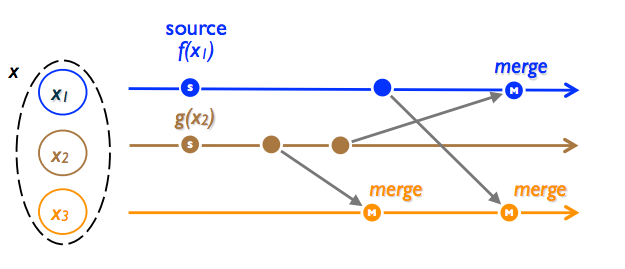
\includegraphics[height=3cm]{media/crdt}\label{fig:CRDT Sample}
\end{frame}
